\documentclass[12pt,a4paper,twoside]{article}
\usepackage{polski}
\usepackage[utf8]{inputenc}
\usepackage[left=3.5cm,right=2.5cm,top=2.5cm,bottom=2.5cm]{geometry}
\usepackage{graphicx}
\usepackage{lipsum}
\usepackage{setspace}
\usepackage{xcolor}
\spacing{1.15}
\setlength{\parindent}{1.25cm}
%% ########################################################
\begin{document}
\thispagestyle{empty}
\begin{center}

\includegraphics[width=\textwidth]{img/logo_AGH.jpg}\\
{\bf{\sf WYDZIAŁ GEOLOGII, GEOFIZYKI I OCHRONY ŚRODOWISKA}}\\[5mm]
%% ======================================================
{\bf{\sf{KATEDRA GEOINFORMATYKI I INFORMATYKI STOSOWANEJ}}}\\[14mm]

{\sf{\huge Projekt dyplomowy}}\\[12mm] 
%% ======================================================
{\sf{\Large Aplikacja do zarządzania zbiorami danych\\[2mm] 
Dataset management application}}\\[40mm]
\end{center}
{\sf\begin{tabular}{ll}
	Autor: & Monika Hertel\\
	Kierunek studiów: & Inżynieria i Analiza Danych\\
	Opiekun pracy: & dr Paweł Oleksik\\
\end{tabular}}\\[10mm]
\begin{center}
{\sf Kraków, 2024}
\end{center}
%% ########################################################
\newpage
\tableofcontents
\newpage
\section*{Wstęp}
\addcontentsline{toc}{section}{Wstęp}
{\color{blue}{(Tutaj niedługo powstanie wstęp)}}\par
\subsection*{Cel i zakres projektu}
Projekt ma na celu przedstawienie możliwości systemu ułatwiającego użytkownikowi proces zbierania i segregowania informacji. Poniższa praca skupi się na ogólnym koncepcie aplikacji oraz szczegółowym opisie implementacji modułu tworzącego streszczenia.
\newpage
%% ########################################################
\section{Zagadnienia teoretyczne}
%% ########################################################
\subsection{Problem tworzenia streszczeń}
%%(JA TUTAJ ROBIĘ NIENADZOROWANY TEXTRANK JAK COŚ)\\
Streszczenie w każdej pracy naukowej jest jej ważną częścią. Osoby poszukujące informacji na dany temat nie są w stanie przetworzyć ilości dostępnych informacji. Ma ono na celu przekazać kluczowe informacje o czytanym dokumencie, aby czytelnik mógł ocenić czy dany artykuł zawiera informacje mu przydatne. \par
W kontekście uczenia maszynowego kondensowanie treści, w celu stworzenia kontekstu, opiera się o obliczanie poziomu istotności dla każdego zdania. \cite{MUTLU2020102359}. Automatyzacja tego procesu dąży do ułatwienia autorom tworzenia prac, poprzez skrócenie czasu, którego wymaga kreacja abstraktu. Systemy ATS (ang. \textit{Automatic Text Summarization}) są jednym z cięższych wyzwań sztucznej inteligencji, dotyczących przetwarzania języka naturalnego \cite{ELKASSAS2021113679}. Podejścia do tworzenia tych systemów, możemy podzielić na ekstraktywane, abstrakcyjne i hybrydowe. 
\subsubsection{Metody ekstraktywne a abstrakcyjne}
Większość badań nad systemami ATS skupia się na użyciu metod ekstraktywnych, starając się przy tym uzyskać zwięzłe i kompletne streszczenia. Podejście ekstraktywne polega na wybraniu najważniejszych zdań z całego dokumentu, a długość uzyskanego wyniku zależy od wartości stopnia kompresji \cite{Gambhir2017}. \par
Streszczenia stworzone z użyciem metod abstraktywnych zawierają zdania, które nie znajdują się w orginalnym tekście. System musi w pewnym stopniu ``rozumieć'' tekst, aby móc poprawnie zinterpretować dokument. Abstraktywność wymaga implementacji bardziej złożonych algorytmów przetwarzania języka naturalnego.\par
Istnieje również podział zadania podsumowania na nienadzorowane i nadzorowanie. Nienadzorowane tworzą streszczenia tylko na podstawie danych wejściowych, czyli jedynie zawartości wprowadanego dokumentu. Do optymalnego wyboru zdań, takie systemy implementują metody natury heurystycznej. Z tego powodu są one odpowiednie do przetwarzania danych na bierząco.\par
Sposób nadzorowany wymaga przeprowadzenia fazy trenowania modelu, która wymaga wprowadzenia opisanego zbioru treningowego. Takie zbiory powinny posiadać docelowe postacie streszczeń otrzymane z pełnego tekstu dokumentu. Taki proces jest trudny do przeprowadzenia na większej ilości tekstów.
\subsubsection{Ocena poprawności abstraktu}
Zazwyczaj ingerencja człowieka jest wymagana przy ewaluacji wytworzonego streszczenia. Treść jest sprawdzana pod kątem poprawności gramatycznej, składni czy całościowej spójności. Taka ewaluacja wymaga dużego nakładu pracy, a przy większych projektach jest praktycznie niemożliwe. Dlatego możliwość zautomatyzowania tego procesu jest wręcz wymagana.\par
Jednymi z pierwszych metod ewaluacji automatycznej były metryki takie jak podobieństwo cosinusowe (\textit{ang. cosine similarity}), \textit{unit overlap} czy miara najdłuższego wspólnego podzdania (\textit{ang. longest common subsequence}). Te elementy zostały później skondensowane w zbiór kryteriów opisanych akronimem \textit{ROUGE} (\textit{ang. Recall-Oriented Understudy of Gisting Evaluation}) \cite{rouge}. Poniższy segment przedstawia poszczególne komponenty zestawu \textit{ROUGE}, to jest kryteria \textit{ROUGE-N}, \textit{ROUGE-L} oraz \textit{ROUGE-S}.\par
\textit{ROUGE-N} mierzy poziom pokrycia n-gramów, czyli ciągłych sekwencji \textit{n} słów, pomiędzy wytworzonym tekstem a tekstem źródłowym. Najczęstszym przypadkiem użycia tego kryterium jest ewaluacja poprawności gramatycznej. Miary \textit{ROUGE-1} oraz \textit{ROUGE-2} należą do miar \textit{ROUGE-N} i w kolejności kożystają z unigramów i bigramów.
Tymczasem \textit{ROUGE-L} jest wyznaczana na podstawie porównania najdłuższych wspólnych sekwencji słów w zdaniach, występujących w streszczeniu wygenerowanym i wzorcowym. \textit{ROUGE-S} działa na tej samej zasadzie co \textit{ROUGE-2} lecz uwzględnia w swoim działaniu struktury skip-bigram, który jest rozszerzeniem definicji bigramów o możliwość zawierania w sobie maksymalnie jednego przedimka.
%% ########################################################
\subsection{Tworzenie aplikacji webowych}
{\color{blue}{(pomysł)}}\par
%% ########################################################
\subsection{Ekstrakcja tekstu plików PDF}
Pliki PDF są powszechnie przyjętym standardem przechowywania informacji. Format PDF jest oparty o strukturę binarnego formatu plików, zoptymalizowanego pod kątem wysokiej wydajności odczytu wizualnego. Zawierają w sobie informacje o strukturze dokumentu, takie jak zawartość tekstowa, grafiki czy użyta czcionka. Są one zoptymalizowane pod drukowanie. Niezaszyfrowane PDF mogą być w całości reprezentowane z użyciem wartości bitowych, odpowiadających części zbioru znaków zdefiniowanego w \textit{ANSI X3.4-1986}, symbole kontrolne oraz puste znaki. Wizualnie jednak nie są one ograniczone do zbioru znaków ASCII.\par
Format PDF separuje informacje dotyczące samego znaku a jego wizualną reprezentacją. Jest to rozróżnienie na znak pisarski i glif, gdzie grafem jest jednostką tekstu a glif, jednostką graficzną. Glif informuje o położeniu znaków na stronie dokumentu, jego czcionce i innych elementach wyglądu. \par
Otrzymanie zawartości pliku może być wykonane za pomocą wydobycia elementów PDF z strumienia pliku lub z użyciem analizy obrazów, na przykład technologi optycznego rozpoznawania znaków OCR (\textit{ang. Optical Character Recogintion}). 
Podstawowym zadaniem systemu OCR jest konwersja dokumentów w dane możliwe do edytowania czy wyszukiwania. Techniki oparte o analizę obrazów są bezpośrednio zależne od jakości wprowadzonego elementu. Idealną sytuacją dla wykożystania metod OCR jest kiedy posiadany plik zawiera w sobie jedynie tekst i jest obrazem binarnym \cite{mithe2013optical}. Dodatkowym atutem takich systemów jest możliwość wykrycia pisma i konwersja na tekst.\par
Ekstrahowanie danych z strumienia pliku, wiąże się z kilkoma problemami. Biorąc pod uwagę możliwość że plik pdf może posiadać różne kodowanie takie jak \textit{UTF-8}, \textit{ASCII} czy \textit{Unicode}, możemy doświadczyć utraty informacji spowodowanej schematem kodowania pliku. Automatyczna ekstrakcja zawartości polega na selekcji znaków znajdujących się pomiędzy zdefiniowanymi słowami kluczowymi. Pliki PDF są przystosowane do drukowania, z tego powodu reprezentacja tekstu w strumieniu może się znacząco różnić od tej na stronie. Ponieważ pozycje znaków na poszczególnych stronach są absolutne, przedstawienie w strumieniu bierze pod uwagę spacje między elementami.\par
Niezależne od sposobu pobierania informacji, nie jest możliwe zagwarantowanie ich poprawności względem dokumentu wejściowego. Brak formalnej definicji struktury, przynajmniej jeżeli chodzi o artykuły naukowe, uniemożliwia stworzenie uniwersalnego algorytmu ekstrakcji.
\newpage
\section{Implementacja}
\subsection{Projekt systemu}
Aplikacja została zaprojektowana z myślą o użytkownikach będących w posiadaniu dużej ilości plików z danymi. Głównym celem jest automatyzacja procesu segregowania i przetwarzania informacji. System etykietuje otrzymane pliki poprzez ekstrakcje słów kluczowych i daje możliwość wyszukiwania plików w bardziej optymalny sposób. Otrzymane dokumenty są kategoryzowane ze względu na słowa klucze. Po otrzymaniu elementów o podobnej strukturze i zawartości, są one łączone ze sobą. Informacja o takim połączeniu jest umieszczana w bazie danych, tak aby przy odczycie jednego z elementów, drugi był sugerowany jako następny plik do wyświetlenia. \par
%% ########################################################
\subsection{Architektura systemu} %omg electron+react+flask
Aplikacja została zbudowana z myślą o zapewnieniu interfejsu użytkownika przy użyciu JavaScript React, serwera HTTP opartego na Flask Python, oraz bazy danych MongoDB, która jest bazą typu NoSQL. Zintegrowana całość jest uruchamiana z wykorzystaniem pakietu Electron, co umożliwia stworzenie aplikacji natywnej, zachowując przy tym funkcje przeglądarki oraz pozwalając na dostęp do zasobów systemowych.\par
Zakres implementacji obejmuje stworzenie serwera działajacego w oparciu o protokół HTTP. Serwer zwraca odpowiedz w postaci pliku JSON, który następnie jest przetwarzany przez stronę React, czego wynik jest wyświetlany klientowi.\par
\begin{figure}[h!]
\centering
  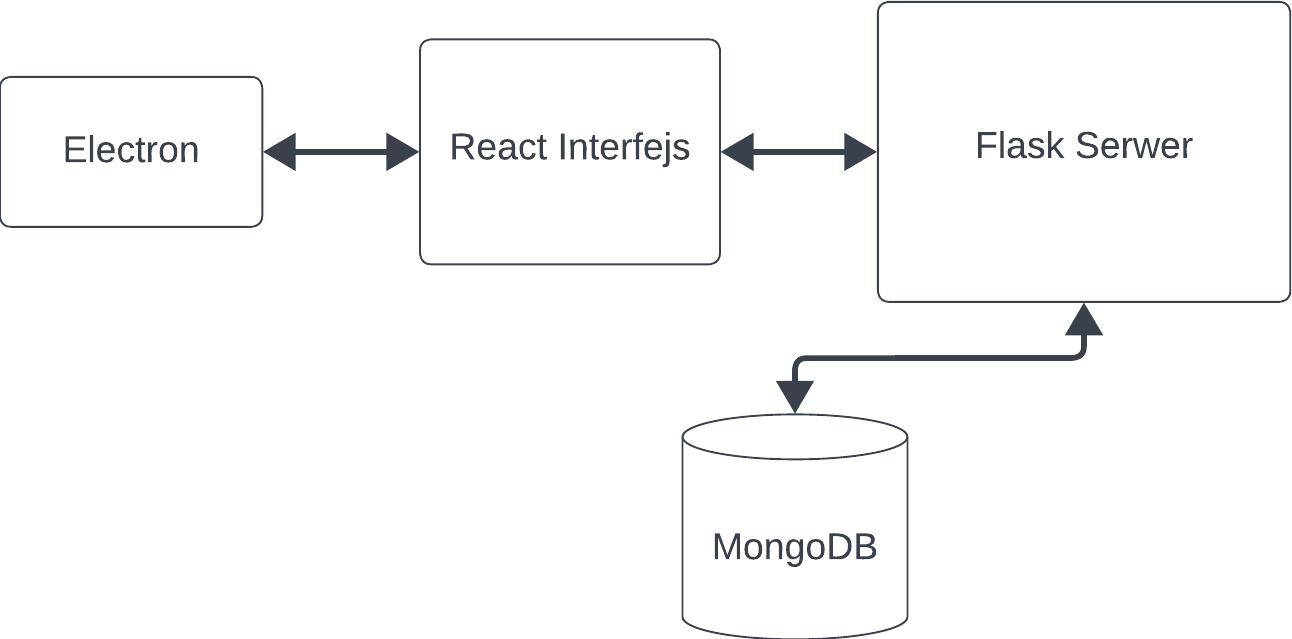
\includegraphics[width=\textwidth]{img/archi.png}
  \caption{Diagram łączenia komponentów}
\end{figure}
%% ########################################################
System składa się z 4 głównych komponentów:
\begin{enumerate}
	\item serwer HTTP
	\item baza danych
	\item interfejs użytkownika
	\item konwerter na aplikację natywną
\end{enumerate}
\subsubsection{Javascript React}
Jest to biblioteka pozwalająca na budowanie interaktywnych interfejsów użytkownika. Główną koncepcją React są komponenty, czyli samodzielne, hermetyczne jednostku interfejsu. Pozwala to na reakcje na zmiany wywołane przez użytkownika lub sam system i przy tym automatyczne aktualizowanie tych stron. React używa składni JSX (\textit{Javascript XML}), który jest rozszerzeniem składni Javascript. Integruje ona kod Javascript z deklaratywnym opisem struktury interfejsu.
\subsubsection{Python Flask}
Flask to lekki i elastyczny framework, pozwalający na szybkie tworzenie aplikacji internetowych przy minimalnej ilości kodu. Dostarcza on jedynie niezbędne narzędzia, stawiając tym na dużą swobodę implementacji innych funkcji. 
Funkcja serwera jest uruchamiana w sytuacji gdy na podany adres URL zostanie wysłany komunikat. Informacja o aktywującym adresie jest przekazywana z użyciem dekoratora \textit{.route()}. Rysunek X przedstawia przykład takiego wywołania.\par
Jedną z możliwość tej biblioteki jest generowanie plików strony jako wynik końcowy działania funkcji. Kożystamy w takiej sytuacji z metody \textit{render\_template()}, która otrzymuje na wejściu uprzednio utworzony szablon HTML.\par 
Implementacja serwera z pomocą pakietu Flask umożliwia kożystanie z szerokiego spektrum bibliotek dotyczących sztucznej inteligencji.
\begin{figure}[h!]
\centering
  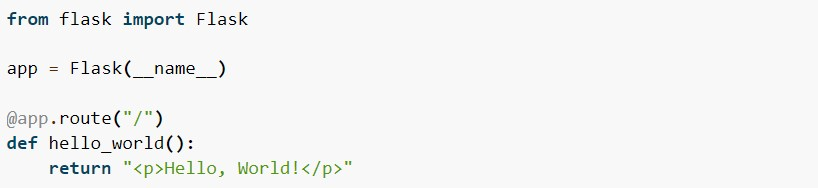
\includegraphics[width=\textwidth]{img/flask.jpg}
  \caption{Przykładowa implementacja funkcji serwera}
\end{figure}
\subsubsection{Electron}
Biblioteka Electron jest projektem open-source umożliwiającym tworzenie aplikacji natywnych używając technologii web. Standard tworzenia aplikacji z pomocą tej biblioteki jest oparty o komunikację międzyprocesową (\textit{ang. IPC, Inter-process communication}), która jest wynikiem implementacji izolacji kontekstu. Izolacja kontekstu odpowiada za separację procesu renderowania strony od głównego procesu aplikacji w środowisku Node.js. Zwiększa to bezpieczeństwo aplikacji, negując możliwość dostępu do użytych API z strony. \par
System posiada jeden główny proces \textit{``main''}, którego celem jest tworzenie aplikacji i kierowanie podprocesami, oraz wiele procesów odpowiedzialnych za renderowanie zawartości strony zwanych procesami \textit{``renderer''}. Biblioteka umożliwia również dodanie skryptów, które działają przed renderowaniem strony (ang. \textit{preload scripts}). Otrzymują one dodatkowe możliwości w porównaniu plików \textit{renderer}, poprzez posiadanie uprawnień do korzystania z Node.js APIs. Mogą one bezpiecznie udostępnić części API dla procesów strony.
%\begin{figure}[h!]
%\centering
%  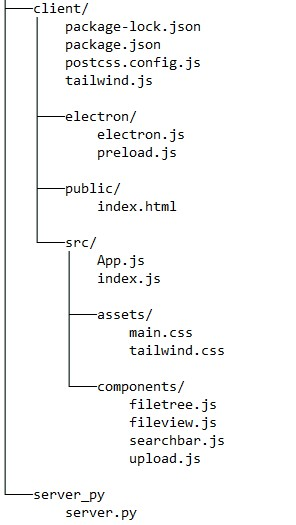
\includegraphics{img/file_structure.jpg}
%  \caption{Uogólniona struktura projektu}
%\end{figure}
%\newpage
%% ########################################################
\subsection{Obsługiwane rodzaje plików}
%% ########################################################
System jest przystosowany do obsługi plików o rozszerzeniach takich jak \textit{PDF}, \textit{CSV} i \textit{TXT}. Każdy rodzaj pliku ma osobne funkcjonalności opisane poniżej. Do plików przypisujemy tag opisujący rodzaj pliku, lecz nie jest on odrębną jednostką od słów kluczowych generowanych na podstawie zawartości pliku.
\subsubsection*{Pliki PDF}
Proces obsługi plików pdf jest zależny od wielu czynników. Najprostrzymi plikami do analizy są artykuły posiadające zakładki (\textit{ang. outlines}) o ujednoliconej strukturze, zawierające jedynie tekst. \textit{Outlines} są potrzebne do ustalenia tytułu danego pliku, ponieważ nie zawsze nazwa samego pliku koresponduje tytułowi.\par
System wykorzystuje potokowanie zawartości w celu ekstrakcji tekstu, obrazów oraz tabel. Działanie aplikacji jest oparte o sam tekst pliku co Na potrzeby aplikacji, takie fragmenty jak tabele czy grafiki są jedynie przeszkodą , ponieważ nie powinne one wpływać na wynik algorytmu streszczania. Część elementów tabelarycznych jest niepoprawnie podpisywana jako tekst, co może przyczynić się do generacji niezrozumiałych streszczeń. 
\subsubsection*{Pliki tabelaryczne CSV}
Podstawowym zachowaniem aplikacji w obliczu plików zawierających dane tabelaryczne w systemie przecinkowym generacja opisu zgodnie z następującymi krokami. Dla każdej kolumny pobierana jest jej nazwa oraz rodzaj danych zawartych w niej (\textit{double}, \textit{string}, itp.). \par
Ze względu na rodzaj pliku generacja słów kluczy może przebiec na dwa sposoby: tagami zostają nazwy kolumn lub użytkownik samodzielnie je dodaje. Oba podejścia mają swoje wady. Nazwy kolumn nie są wymagane podczas kreacji tabel, więc tworzenie tagów w takiej sytuacji nie jest optymalne. Drugie podejście wymaga od użytkownika większego wkładu w ten proces. Potrzebna do tego jest pewna znajomość zestawu danych, który chcemy wprowadzić do systemu aby odpowiednio przypisać słowa klucze do plików.
\subsubsection*{Pliki tekstowe TXT}
Zawartość plików tekstowych nie jest uwarunkowana żadnymi normami, co czyni obsługę tych plików niemożliwą do standaryzacji. Podczas dodawania do aplikacji, wymagają one od użytkownika określenia rodzaju zawartości. Opcjami, które użytkownik ma do wyboru są: tekst lub dane tabelaryczne.\par
W pierwszym przypadku program sprawdza długość tekstu i na tej podstawie decyduje o następnych krokach. Domyślną długością graniczną jest 200 słów, lecz może ona być ustawiona manualnie przez klienta. Po przekroczeniu tego progu, system procesuje plik w sposób podobny do obsługi plików \textit{PDF}. Tworzone jest streszczenie.\par
\newpage
\subsection{Schematy poszczególnych funkcjonalności}
%%s(dodać screeny z postmana jak wywołuje jakąś funkcje)
%%Poniżej zaprezentowane są funkcjonalności końcowej aplikacji na przykładzie plików o rozszerzeniu PDF oraz diagram aktywności aplikacji.
%%(można zrobić opisy funkcjonalności, nawet tych nie zaimplementowanych razem ze schematami, a potem cały opis modułu streszczeń)
\subsubsection{Dodawanie pliku PDF}
Zachowanie systemu przy dodaniu plików tekstowych.
\begin{enumerate}
	\item Gdy użytkownik wybierze plik, aplikacja przesyła ścieżkę pliku do serwera,
	\item System ekstraktuje z pliku całą zawartość z pomocą biblioteki języka Python \textit{PdfMiner},
	\item Z zawartości zostają wyciągnięte słowa klucze. Tworzenie tzw. tagów odbywa się z pomocą biblioteki \textit{yake} oraz metody \textit{KeywordExtractor()}. Przyjmuje ona następujące parametry:
	\begin{itemize}
		\item \textit{lan} - język danego tekstu,
		\item \textit{n} - maksymalna ilość słów w jednym tagu,
		\item \textit{deduplim} - szansa na powtóżenie się słów w różnych słowach kluczach,
		\item \textit{top} - ilość elementów wyjściowych
	\end{itemize}
	\begin{figure}[h]
		\centering
  		\includegraphics[width=\textwidth]{img/yake\_keyword.jpg}
  		\caption{Przykład użycia \textit{KeywordExtractor()}}
	\end{figure}
	\item w tym samym czasie z pomocą biblioteki \textit{sumy} oraz funkcji \textit{TextRankSummarizer}, jest tworzone streszczenie z użyciem algorytmu \textit{TextRank},
	\item jeżeli plik pdf posiada zakładki (ang. \textit{outlines}) to metoda \textit{.get\_outlines()} ekstraktuje je i z wyniku możemy otrzymać tytuł dokumentu i nadać plikowi taką nazwę. a jeżeli ich nie ma to tytułem pliku zostaje bazowa nazwa pliku,
	\item ostatecznie wszystkie informacje są zbierane i przesyłane do bazy danych.
\end{enumerate}
%\begin{figure}[h]
%\centering
%  \includegraphics[width=\textwidth]{img/file\_add\_pl.png}
%  \caption{Schemat sekwencyjny dodawania pliku}
%\end{figure}\par
Model TextRank zastosowany w projekcie, jest algorytmem rankingowym opartym na grafach \cite{textrank}. Operuje on na zasadach ``głosowania'' i ``rekomendacji''. Jest on używany do tworzenia streszczeń metodą ekstraktywną i nienadzorowaną. Dla naszego systemu, nie jest możliwe wytworzenie odpowiedniego zbioru treningowego, aby móc zastosować metody nadzorowane. \par
Biblioteka \textit{PdfMiner} języka Python
\begin{figure}[h!]
\centering
  \includegraphics{img/activity\_diagram.png}
  \caption{Diagram aktywności przesyłania pliku}
\end{figure}
\subsubsection{Wyszukiwanie i wyświetlanie plików}
Użytkownik ma możliwość wysukiwania plików po słowach kluczach lub tytule pliku. Tutaj przydatne jest użycie API generującego synonimy dla wyszukiwanego słowa. System zachowuje się w poniżej opisany sposób.
\begin{enumerate}
	\item aplikacja przesyła komunikat z wyszukiwanym słowem,
	\item serwer używając API synonimów pobiera 5 najbliższych słów do słowa szukanego przypisując im ranking,
	\item serwer przesyła osobne komunikaty do tabeli \textit{file\_properties} w naszej bazie danych, zawierające osobno słowo klucz oraz synonimy
	\item baza zwraca informacje dotyczące znalezionych dokumentów oraz słowo klucz,
	\item serwer zwraca listę plików użytkownikowi, posortowane zgodnie z rankingiem
\end{enumerate}
\begin{figure}[h!]
\centering
  \includegraphics[width=\textwidth]{img/file\_search.png}
  \caption{Schemat sekwencyjny wyszukiwania pliku}
\end{figure}
\newpage
\subsubsection{Asocjacja plików o podobnej tematyce}
Poniższa sekcja przedstawia proces łączenia dokumentów na podstawie wygenerowanych słów kluczowych. System z każdym dodanym plikiem przeszukuję przestrzeń dokumentów i aktualizuje już utworzone rekordy, w sytuacji dopasowania. Schemat przedstawia tworzenie połączeń dla nowo dodanego pliku.
\begin{enumerate}
\item dla każdego słowa kluczowego, jest pobrana lista ID plików z tabeli \textit{file\_properties}, pod warunkiem dopasowania przynajmniej jednego tagu,
\item następnie obliczany jest współczynnik podobieństwa, którego schemat postępowania jest przedstawiony poniżej:
	\begin{enumerate}
		\item wyznaczana jest wartość dla poszczególnych słów kluczy
		\begin{itemize}
			\item jeżeli wysłane słowo kluczowe zgadza się fragmentarycznie z otrzymanym tagiem (np. ``zaburzenia'' a ``zaburzenia odżywiania''), to zapisywana jest wartość $2\cdot\frac{ilosc(dopasowan)}{ilosc\_slow(wejscie)+ilosc\_slow(pobrane)}$,
			\item jeżeli słowa są identyczne, zapisywana jest wartość 1,
		\end{itemize}
		\item wartości dla wszystkich słów kluczy są sumowane i dzielone przez liczbę tagów.
	\end{enumerate}
\item do ID pliku przypisana jest wartość podobieństwa, i po posortowaniu od największej wartości, ID są dodawane do jednego rekordu w tabeli \textit{file\_connections}
	\begin{itemize}
		\item jeżeli wartość podobieństwa nie przekracza 0.3, to plik nie jest brany pod uwagę
	\end{itemize}
\end{enumerate}
\subsubsection{Obsługa plików CSV}
\begin{enumerate}
	\item użytkownik przy dodaniu pliku podaje następujące informacje:
	\begin{itemize}
		\item czy plik zawiera informacje o nazwach kolumn, jeżeli nie to czy chce on nadać te nazwy,
		\item czy słowa kluczowe będą nadane manualnie lub czy powinny być pobrane z nazw kolumn,
	\end{itemize}
	\item odpowiednio wczytywana na server do postaci ramki danych (\textit{ang. dataframe}) modułu \textit{pandas},
	\item sprawdzany i zapisywany jest typ wartości w każdej kolumnie oraz obliczony procent ilości wartości brakujących,
	\item dodanie rekordu do bazy danych.
\end{enumerate}
\subsubsection{Obsługa plików TXT}
Przetwarzanie plików tekstowych rozpoczyna się pytaniem o zawartość takiego pliku. Użytkownik dodaje informacje czy plik zawiera w sobie tekst czy dane kolumnowe. Jeżeli jest to tabela, to proces ekstrakcji jest taki sam jak w przypadku plików csv. 
%\newpage
%% ########################################################
\subsection{Testy funkcjonalne}
%Jeżeli chodzi o testowanie tworzenia streszczeń to nie jest możliwa automatyzacja tego. Nie jesteśmy w stanie przewidzieć jakie zdania będą wchodziły w skład wygenerowanego abstraktu. Czynnik ludzki w tym przypadku jest wymagany do oceny poprawności danego algorytmu. (wait to jak oni sprawdzają to przy metodach abstrakcyjnych????)\par
%jak będzie czas to mogę przetestować ocr i tersseract
%% ########################################################
%\subsection{TEMP Idealna aplikacja}
%DOBRA JEŻELI ROBIMY STRESZCZENIA TO ŻEBY NAJPIERW BYŁ NIENADZOROWANY TYP ROBIENIA STRESZCZEŃ A POTEM JAK PODZIELIMY PLIKI NA KATEGORIE TO WTEDY PRÓBOWAĆ ROBIĆ Z DANYMI WEJŚCIOWYMI, CZYLI NASZE WCZEŚNIEJ DODANE PLIKI (THE BLIND LEADING THE BLIND)\par
%jeszcze można wygenerować nasze streszczenia jako osobny plik; wykrywanie języka dokumentu by się przydało
%% ########################################################
\section{Możliwości rozwoju i wykorzystania aplikacji}
Wspomniane funkcjonalności to jedynie początek istnienia tego systemu. \par
\subsection{Ekspansja działań dotyczących danych tabelarycznych}
Aktualny system pozwala na implementacje metod wstępnego przetwarzania danych (\textit{ang. preprocessing}) z wnętrza aplikacji. Preprocessing oznacza zbiór działań miejących na celu obróbkę i przygotowanie danych do dalszej manipulacji. Do takich działań należą usunięcie wartości brakujących, filtracja czy 
\subsection{Implementacja abstrakcyjnego tworzenia streszczeń}
\subsection{Obsługa obrazów}
\subsection{Kategoryzowanie plików względem zawartości}
\subsection{Ulepszenie procesu ekstrakcji tekstu}
%% ########################################################
\section*{Podsumowanie i wnioski}
\addcontentsline{toc}{section}{Podsumowanie i wnioski}
%%W sumie to nie wiem co jest celem tej pracy ani co mam podsumować, 
%% ########################################################
\newpage
\listoffigures
\addcontentsline{toc}{section}{Spis Rysunków}
\addcontentsline{toc}{section}{Bibliografia}
\bibliographystyle{IEEEtran}
\bibliography{biblioteka}
\addcontentsline{toc}{section}{Bibliografia}
\end{document}